\documentclass[11pt, a4paper]{article}

\usepackage{fullpage}
\usepackage{url}
\usepackage{graphicx}
\usepackage{subcaption}
\usepackage{caption}

\begin{document}

\title{\vspace{-2cm}ARM Final Report}
\author{Group 39\\ \small \textit{Thomas Wong, Steven Chen, Nixon Enraght-Moony, Rickie Ma}}

\maketitle
\section{Assembler}
\subsection{Lexer}
We store the start of the current token, and the
current position. When the next charecter can't be added to the current token
kind (determined by where in the lexer source we are), we make a token from 
start to current, and then set start to current.
\par
This means that each Token doesn't store an owned string of its value, but
rather a pointer into the original source and a length. Because these are not
null terminated, this caused a lot of pain at first, as we coundn't use C's
string functions, so we ended up puting \textbf{ptr+len} into it's own struct, and
writing a string library just for it. This worked well, as we could share it 
with the Symbol Table.
\par
Tokens also sort their kind (A \texttt{enum TokenKind}), and their line and
column. To support this, the lexer must know where it is at all times. It knows
this because it only increments \textbf{current} in on function (\texttt{advance}), so
this function can check if the next char is a
\texttt{\textquotesingle{}\textbackslash{}n\textquotesingle{}}.

\begin{center}
  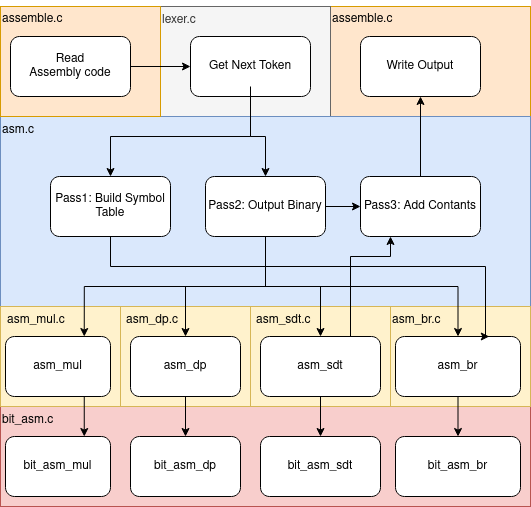
\includegraphics[scale=0.4]{report/asm_arch.png}
\end{center}
\subsection{Stucture}
We have chosen to implement the assembler in \textbf{2-pass}, since it requires less memory, \textit{i.e.} a list of forward addressesses was not required to be maintained.
\begin{itemize}
  \setlength\itemsep{0em}
  \item \texttt{asm.c} contains utility functions for the 4 \texttt{asm\_\*.c} files. The most-used function is \texttt{asm\_expect}, which expects a token received from the \textbf{Lexer} to have the matching of \textbf{TokenKind}, and then return the token. However, if it is not matched, the assembler error will be evoked. Not only does it get the next Token from the \textbf{Lexer}, but it also ensures that the assembly code follows the specified syntax. When the next Token received could be one of the 2 \textbf{TokenKind}, we use \texttt{asm\_match}, where it returns true only if \textbf{TokenKind} is matched, then return the token to the given token pointer. By using this function with if statement, instructions such as \verb|add r1, r2, r3{, <shift>}| are possible to assemble.
  \item  We structured the code such that each type of instuction uses a different C file, this improves code readability and allow parallel coding. \texttt{asm\_dp.c} are used to assemble data processing instructions. \texttt{asm\_mul.c} are used to assemble multiply instructions. \texttt{asm\_sdt.c} are used to assemble single data transfer instructions. \texttt{asm\_br.c} are used to assemble branch instructions.
  \item \texttt{bit\_asm.c} contains functions used for creating the binary representation of the instruction by passing the required arguments such as register number.
  \item  Most of the enum \textbf{TokenKind} are self-explanatory. However, \texttt{TOKEN\_IDENT} could mean instruction kind, register name or shift type. Therefore, it's up to the programmer to handle it correctly. Another way to implement this is to check the token against the list of names in all 3 types, although it improves the readability of the code, it will lower the performance.
  \item  On every new line, the lexer will break down the first token into the Instruction kind and the condition, which is store in a struct, \textbf{InstrCommon}, so that these attributes can be retrieved with ease when passing to \textbf{asm\_*} functions. 
\end{itemize}
\section{Extension}
We have implemented two different extensions, a \textbf{disassembler} and a \textbf{debugger}.
\subsection{Disassembler}
The disassembler translates machine code into \textbf{ARM11} assembly.
\subsubsection{Usage}
The program takes in one \textbf{binary file} and prints out the binary instructions line by line in hexadecimal along with its \textbf{assembly} command. More detail including examples are included in the extension documentation.\\
Here is an example of the disassembler running:
\begin{verbatim}
$ ./disassemble arm11_39/arm11_testsuite/test_cases/ldr09 
000: e59f2008 
ldr r2, [pc, #8] 
001: e2821002 
add r1, r2, #0x2 
002: e3330002 
teq r3, #0x2 
003: 00000000 
andeq r0, r0, r0 
\end{verbatim}
\subsubsection{Structure}
The stucture of the \textbf{disassembler} is simliar to the \textbf{emulator}, whereas the \texttt{disassemble.c} parses in the instructions to the \texttt{dis.c} and is then distributed into the 4 corresponding functions (\textbf{dis\_sdt}. \textbf{dis\_br}, \textbf{dis\_dp}, \textbf{dis\_mul}) according to the \textbf{OpType}. The \textbf{assembly} commands are printed out directly from these functions.
\subsubsection{Challenges}
The hardest parts of the implementation are the \textbf{data processing} and \textbf{single data transfer} instructions, and it holds true for both the \textbf{emulator} and the \textbf{assembler} as well. 

When dealing with \textbf{data processing instructions}, there are commands with 3 arguments and some with 2 arguments, in which there are also special cases involving shifting (test case \texttt{opt\_ldr10}). It was dealt with extra caution and continuous testing.

\subsection{Debugger}
The debugger can halt the execution of the assembly file when a breakpoint is hit, examine the values of registers and step through the commands line by line. It also supports the feature of peeking the next instruction and deleting set breakpoints.
\subsubsection{Usage}
The program takes in one \textbf{ARM11 assembly file} (.s). Commands can be then entered into the prompt.\\ Similar to the \textit{GNU} debugger, the commands are:
\begin{itemize}
  \setlength\itemsep{0em}
  \item \texttt{r}(un/continue), halt the program when a breakpoint is reached.
  \item \texttt{s}(tep), step through the current instruction.
  \item \texttt{q}(uit), quit the debugger.
  \item \texttt{b}(reak) \texttt{\#x}, set a breakpoint on line \texttt{x} of the \textbf{assembly file}.
  \item \texttt{d}(elete) \texttt{\#x}, delete breakpoint \texttt{x}.
  \item \texttt{p}(rint) \texttt{reg}, print the content of register \texttt{reg}.
  \item \texttt{l}(ine) \texttt{n}(ext), print the next instruction.
\end{itemize}
Here is an example of the debugger running:
\begin{verbatim}
$ ./debug arm11_39/arm11_testsuite/test_cases/loop03.s
> b 3
Breakpoint 1 set at line 3 (instruction 2).
> r
Breakpoint 1 at Line 3
Next Instruction at Line 3: 
002: e3520000
cmp r2, #0x0
> s
Previous Instruction at Line 3: 
002: e3520000
cmp r2, #0x0
Next Instruction at Line 4: 
003: 1afffffc
bne #0x4
> p r2
9
> r
Breakpoint 1 at Line 3
Next Instruction at Line 3: 
002: e3520000
cmp r2, #0x0
> q
\end{verbatim}
\subsubsection{Structure}
\begin{center}
  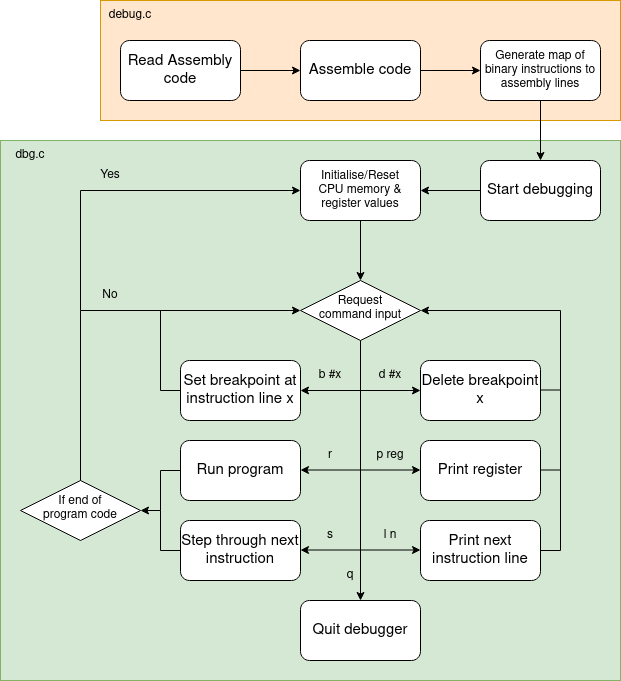
\includegraphics[scale=0.4]{report/dbg_arch.png}
\end{center}
The debugger first assembles the assembly code in \path{debug.c}, then parses the map of \textit{binary instructions - assembly line} pair to the \path{dbg.c}.

The main sequence of the debugger is shown as in \path{dbg.c} above, which stays in a loop if \textbf{quit} is not triggered.

All other parts of the project (\textbf{assembler}, \textbf{emulator} and \textbf{disassembler}) have been used in this extension to some extent. As a result, code sharing across the project has been done extensively. For instance the \texttt{select\_func} function in \path{emu.c} is used in the \path{dbg.c}.

\subsubsection{Challenges}
This implementation wasn't very difficult to implement, since it shares quite a lot of common code with other parts of the project. However, we still ran into some difficulties, such as IO logic, and choosing the best design approach to maximise function sharing with other functions.

Since the \textbf{assembly} file does not correspond to the \textbf{binary} file line by line, we had to introduce subpograms and mapping to match the \textbf{assembly} file line to its machine code. This involves some adjustments and adaptations from the \path{asm.c}.

\subsection{Testing}
An extensive testsuite, and runner written in \textbf{Go}, can be found in \path{/tests/dbg}. This has test cases for \textbf{debugger}, \textbf{assembler} errors, additional \textbf{assembler} cases (mainly found by \textbf{fuzzing}), and test for the \textbf{debugger}, which we drive programmatically, despite being an interactive program.
\par
One challenge that came up, was that initialy all the \textbf{debugger} output would come at the end, so we couldn't tell what came from which input. This was because \texttt{glibc} won't flush \texttt{stdout} as often when not connected to a TTY. This was frustrating to debug, because the behaviour only occured when connected to the test runner, but not under \texttt{strace} or \texttt{gdb}, but eventually it was solved with \texttt{fflush}.

\textit{Sidenote:} To run the test, ensure \textbf{Go} version 1.18 is installed, \texttt{make test} under \path{\tests} directory. 
\section{Reflection}
As a group we have improved our work splitting, by having two people tackling on the assembler and the other two working on the debugger. Members that had lesser work in the emulator had an increase of workload, and as a team, we were more productive than before.  

As of before, we would mainly meet face-to-face as we thought this is the easiest and the most effective form of communication. Normally we distribute work and discuss ideas physically, but most of the code is written remotely and reviewed online via merge requests. Some issues regarding the project were raised through GitLab as well. 

Overall, I think our group collaborated quite well. In future projects, we would keep the git discipline shown in this assignment, as we did not run into any major problems with git. Also, the way of how we structured our project can be reused, as it is very easy to navigate around different files. 

However, if we were to redo the whole project again, we would meet more in person. Due to issues such as striking, we were not able to meet face-to-face at the very late stage of the project, which reduced our productivity. Also, we would improve our time management, as we had lots to do on the last week of the assignment compared to the week before the C final test.
\subsection{Nixon Enraght-Moony}
While the project went well, we could have done alot better on time management, as we had quite alot of crunch in the last couple of days. Next time, I'd like to be able to spend more time polishing and documenting the code.
\par
Additionaly, while the text runner worked great, I regret using go. It's not that commonly availible (not on lab machines), and in some distros (Ubuntu 20.04) it's very out of date. Combine this with the fact that the CLI interface isn't stable, and it was not a fun time for anyone.
\par
Most of the other tooling worked great: The makefile was setup to automaticly know about headers, recompile when the makefile changed, and to support building with various sanitizers in seperate directories, which was all super helpful.
\subsection{Steven Chen}
I believe that I have fitted nicely in the group as I was able to finish the task that was assigned to me on time. We split the emulator project by instruction type, as being not familiar with C, I was assigned to do the multiply instruction, which is the easiest among the four. This gave me time to improve my skills and learn from my teammates’ codes. After that, I was more confident with my skills and picked up more tasks for the assembler. I have implemented both the data processing instructions and the multiply instructions in the assembler, created some of the utility functions of the assembler and simplifies the code in single data transfer instructions. 

The strength I believe I have is the ability to write clear code which is understandable by other teammates as well as able to understand and simplify others’ code. 

I do have to admit that I have limited knowledge of utility tools in Linux, which has made me work slower than others. However, I am thankful that one of my teammates introduced me to many useful packages such as Capstone and Keystone, which make checking and testing code much easier. 

I believe the way we split the work was excellent, where no one is working on overlapping code so that everyone can work concurrently. I would put more attention on how we split the work in the next project, so the project could be done efficiently. 
\subsection{Thomas Wong}
I have mainly made contributions that are supplementary to my team's code. I have implemented the symbol table used in the assembler using an AVL map. I also introduced assembly file support and added/fixed commands in the debugger.  

I have taken my time to understand the code produced by the group. With that, I have been able to build upon others' code and improve them, this helped me optimise the programs and remove bugs from the project. I have also added suggestions and documented changes I made for better clarity in the relevant files. 

As for weaknesses, I am unfortunately inexperienced in C, which has prevented me from contributing more. I have never used programming languages similar to C before, so it was stressful to have to study the language, start a project and prepare for a test in such a short period of time. Thankfully, I had help from various sources, so I am much more confident in C now. 

Though I had my own projects before, I haven't had the chance to work with others in one. My team has introduced many tools and methods to me, so this project has been a great opportunity to learn how to cooperate in a team. 
\subsection{Rickie Ma}
I think I have fitted in the group quite well. I oversaw the single data transfer and the branching instructions for the emulator, I have also contributed to the data processing and the branching procedures for the disassembler and most of the debugger.  

I am good at understanding other member's code and develop from the foundation, which was proven quite handy in this project. Also, I would produce code that is easily understandable for other collaborators. 

My weakness is lack of knowledge on C. Since I had some previous experience with C++, I thought this language would not be much of a challenge, yet I had to consult an expert in C in our team multiple times for more obscure uses of the language. However, having done this project, I am much more proficient in C.  

If I were in a different team, I would bring the git discipline from this group, as we never had any big issues with our git timeline. 

\end{document}

%%% Local Variables:
%%% mode: latex
%%% TeX-master: t
%%% End:
